% (c) 2002 Matthew Boedicker <mboedick@mboedick.org> (original author) http://mboedick.org
% (c) 2003-2007 David J. Grant <davidgrant-at-gmail.com> http://www.davidgrant.ca
% (c) 2008 Nathaniel Johnston <nathaniel@nathanieljohnston.com> http://www.nathanieljohnston.com
% (c) 2011 Scott Clark <sc932@cornell.edu> http://cam.cornell.edu/~sc932
% (c) 2015 Arne Hassel <arne.hassel@gmail.com> http://icanhasweb.net
%
%This work is licensed under the Creative Commons Attribution-Noncommercial-Share Alike 2.5 License. To view a copy of this license, visit http://creativecommons.org/licenses/by-nc-sa/2.5/ or send a letter to Creative Commons, 543 Howard Street, 5th Floor, San Francisco, California, 94105, USA.

\documentclass[letterpaper,10pt,english]{article}
\newlength{\outerbordwidth}
\pagestyle{empty}
\raggedbottom
\raggedright
\usepackage{babel}
\usepackage{float}
\usepackage[T1]{fontenc}
\usepackage{framed}
\usepackage{gfsartemisia-euler}
\usepackage{graphicx}
\usepackage[utf8]{inputenc}
\usepackage{tabularx}
\usepackage{tocloft}
\usepackage{url}
\usepackage[svgnames]{xcolor}
\usepackage{wrapfig}

%-----------------------------------------------------------

%Edit these values as you see fit

\setlength{\outerbordwidth}{3pt}  % Width of border outside of title bars
\definecolor{shadecolor}{gray}{0.75}  % Outer background color of title bars (0 = black, 1 = white)
\definecolor{shadecolorB}{gray}{0.93}  % Inner background color of title bars}

%-----------------------------------------------------------

%Margin setup

\setlength{\evensidemargin}{-0.25in}
\setlength{\headheight}{-0.25in}
\setlength{\headsep}{0in}
\setlength{\oddsidemargin}{-0.25in}
\setlength{\paperheight}{11in}
\setlength{\paperwidth}{8.5in}
\setlength{\tabcolsep}{0in}
\setlength{\textheight}{9in}
\setlength{\textwidth}{7in}
\setlength{\topmargin}{-0.3in}
\setlength{\topskip}{0in}
\setlength{\voffset}{0.1in}

%-----------------------------------------------------------

%Custom commands

\newcommand{\resitem}[1]{\item #1 \vspace{-2pt}}

\newcommand{\resheading}[1]{\vspace{8pt}
  \parbox{\textwidth}{\setlength{\FrameSep}{\outerbordwidth}
    \begin{shaded}
\setlength{\fboxsep}{0pt}\framebox[\textwidth][l]{\setlength{\fboxsep}{4pt}\fcolorbox{shadecolorB}{shadecolorB}{\textbf{\sffamily{\mbox{~}\makebox[6.762in][l]{\large #1} \vphantom{p\^{E}}}}}}
    \end{shaded}
  }\vspace{-5pt}
}

\newcommand{\ressubheading}[4]{
\begin{tabularx}{6.5in}{l@{\cftdotfill{\cftsecdotsep}\extracolsep{\fill}}r}
		\textbf{#1} & #2 \\
		\textit{#3} & \textit{#4} \\
\end{tabularx}\vspace{-6pt}}

%-----------------------------------------------------------

\title{Curriculum Vitae}

\begin{document}

\begin{minipage}{\textwidth}
\begin{wrapfigure}{r}{0pt}
	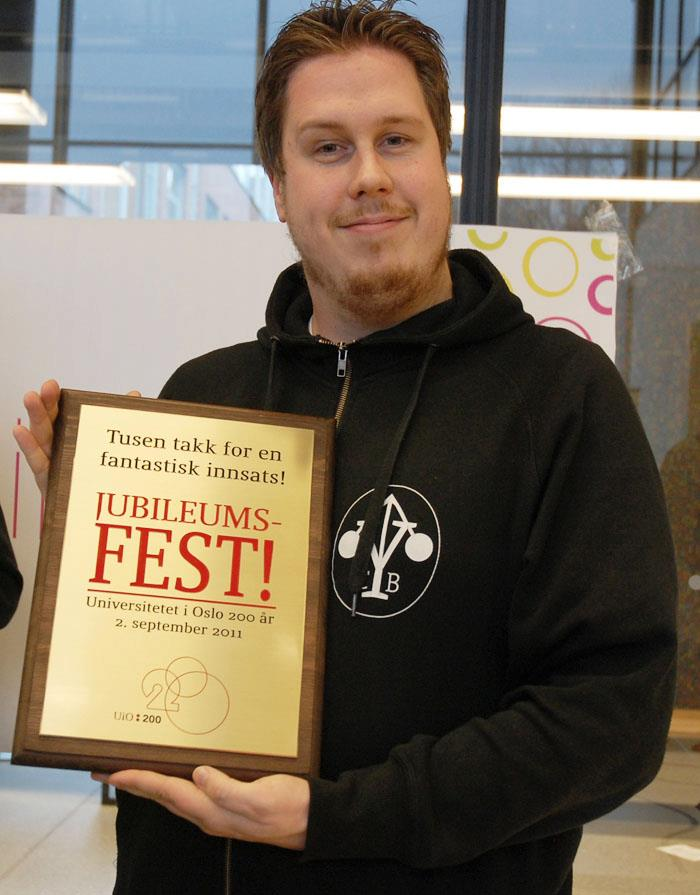
\includegraphics[height=45mm]{uio200.jpg}
\end{wrapfigure}

\textbf{\Large Curriculum Vitae for Arne Hassel}

\vspace{5mm}

\begin{tabular}{p{1in} l}
Adress: & Helgesens gate 12 F, 0553 Oslo, NORWAY\\
Phone: & (+47) 416 94 086 \\
Mail: & \url{arne.hassel@gmail.com} \\
Born: & December 5th 1984 \\
Marital status: & Unmarried \\
\end{tabular}

\vspace{5mm}

\begin{minipage}{5.5in}
Front-end developer in Questback. Graduated master in computer science, bachelor in Economics. Focused on web-based solutions. Experienced programmer, solution oriented and quick to learn new technologies and programming languages.
\end{minipage}

\end{minipage}

\resheading{Work Experience}

\begin{itemize}
\item
	\ressubheading{Questback AS}{Oslo, Norway}{Front-end developer}{2015 - current}
	\begin{itemize}
		\resitem Responsible for the front-end development on Questback Essentials, the DIY survey tool created and developed by Questback
	\end{itemize}
\item
	\ressubheading{Centre for Shared Decision making and Collaborative Care Research}{Oslo, Norway}{System developer}{2008 - 2014}
	\begin{itemize}
		\resitem{Worked mostly frontend (HTML, CSS og Javascript),  but also some backend (.NET)}
	\end{itemize}
\item
	\ressubheading{Senter for Helse \& Arbeid}{Oslo, Norway}{Personal assistant}{2008}
\item
	\ressubheading{Kiwi}{Risør \& Oslo, Norway}{Part-time worker}{1999 - 2008}
\end{itemize}

\resheading{Education}
\begin{itemize}
\item
	\ressubheading{Department of informatics, University of Oslo}{Oslo, Norway}{Master of Computer Science: programming and networks (current)}{2010 - 2012}
	\begin{itemize}
		\item Wrote my master thesis on Javascript and Semantic Web; my supervisors were Kjetil Kjernsmo and Martin Giese
	\end{itemize}
\item
	\ressubheading{Department of informatics, University of Oslo}{Oslo, Norway}{5-year Master, Distributed Systems and Networks}{2007 - 2010}
\item
	\ressubheading{Norwegian University of Life Sciences}{Ås, Norway}{Bachelor in Economics and Administration}{2003 - 2007}
\item
	\ressubheading{Risør VGS}{Risør, Norway}{General studies}{2000 - 2003}
\end{itemize}

\resheading{Certifications}
\begin{itemize}
\item MS: Programming in HTML5 with JavaScript and CSS3 (Microsoft, 2015)
\item MCPS: Microsoft Certified Professional (Microsoft, 2015)
\item Certified ScrumMaster (Scrum Alliance, 2013-2015)
\end{itemize}

\resheading{Skills}

See attached competence chart for more details.

\begin{itemize}
\item {\bf Development:} {\bf (Very good:)} CSS, HTML, Javascript, LESS, Sass, {\bf (Good:)} C\#, SQL, RDF, SPARQL, XML, XSLT
\item {\bf Frameworks/Libraries:} Angular, Knockout, jQuery, .NET MVC (2, 3, 4 \& 5), Umbraco (4 \& 7), Compass
\item {\bf Computer science:} Design patterns, databases, semantic technologies, system development, algorithms, data structures, qualitative research, modeling, computer architecture
\item {\bf Language:} Norwegian (native tongue), english (fluent)
\end{itemize}

\resheading{Selected projects}

\begin{itemize}
\item {\bf hdo-aurelia:} Experimental project that aims to give power-tools to the analysts in Holder de ord. \url{https://github.com/megoth/hdo-aurelia}
\item {\bf ifi-ordenen:} A dynamically generated static HTML webpage that is the official site of Her Majesty the Royal Penguin's order. \url{https://github.com/megoth/ifi-ordenen}
\end{itemize}

\resheading{Voluntary Work and Honorary Positions}

\begin{itemize}
\item
	\ressubheading{Kodeklubben Oslo}{Oslo, Norway}{Code supervisor}{2016 - current}
	\begin{itemize}
		\resitem{Volunteers as code supervisor for a branch of Lær Kidsa Koding in Oslo, that aims to teach children how to code.}
	\end{itemize}
\item
	\ressubheading{Holder de ord}{Oslo, Norway}{Web developer}{2011 - current}
	\begin{itemize}
		\resitem{Contributes to several projects developed and maintained by Holder de ord, \url{holderdeord.no}, a Norwegian political party-independent group consisting of volunteer that strives to create tools enabling the Norwegian people to get an easier insight into the Norwegian Parliament.}
	\end{itemize}
	\ressubheading{Cybernetic Society (CYB)}{Oslo, Norway}{Treasurer, Member of the Sponsor Board, Guard}{2009 - 2012}
\item
	\ressubheading{Birthday Party at Ole-Johan Dahls hus September 2nd}{Oslo, Norway}{Party General/Coordinator (worked with University of Oslo)}{2011}
\item
	\ressubheading{IAESTE}{Ås, Norway}{National Computer Manager, Leader, Treasurerer, Vice Leader}{2003 - 2007}
\item
	\ressubheading{UKA i Ås}{Ås, Norway}{Webmaster, Guard}{2004, 2006}
\end{itemize}

\resheading{Personal details}

\begin{itemize}
\item Have a driver license class B (norwegian)
\end{itemize}

\end{document}
